\documentclass[a4paper]{article}% or something else
\usepackage{pdfpages}    %need this package
\usepackage{tikz}
\usepackage{xcolor}
\usepackage{eso-pic}
\usepackage{ctex}

\usepackage{lscape}
\usepackage{rotating}%宽表格
\usepackage{longtable}%长表格,表格分页
\usepackage{amsmath}%数学
\usepackage{multirow}
\usepackage{hyperref}
%\newcommand{\watermarkpic}[3]{\AddToHook{shipout/foreground}{
\newcommand{\watermarkpic}[3]{\AddToHook{shipout/background}{
\parbox[b][\paperheight]{\paperwidth}{
\vfill%
\centering%
  \tikz[remember picture,overlay]
    \node[rotate=#1,scale=#2] at (current page.center)
 	{\textcolor{gray!70!cyan!30}{#3}};
\vfill}}}
\watermarkpic{30}{5}{热控汽机}

\title{2024年热控汽机检修压力开关校验记录}
\author{热控班组}


\date{\today}
\begin{document}
\maketitle
\begin{landscape}
\begin{longtable}{|c|c|c|c|c|c|c|c|}
\hline
	序号 & 项目名称 & 测点名称 & 测点类型 & 定值 & 延时时间 & 主要逻辑关系 & 备注\endhead
\hline
	&\multicolumn{6}{|c|}{每台汽轮机安装两台联启直流油泵压力开关,每组压力开关常闭点并联接入220VDC控制回路}&\tabularnewline
\hline
1&\href{http://dklovelich.iok.la/taizhang/group_account/look_content.php?id=6586}{1号汽轮机润滑油压力低联启直流油泵}&\parbox[c][12ex][c]{9em}{ 10MAV40CP002\\10MAV40CP003}&压力开关&80KPa&-&2取1& 下NC \tabularnewline
\hline
2&\href{http://dklovelich.iok.la/taizhang/group_account/look_content.php?id=6597}{2号汽轮机润滑油压力低联启直流油泵}&\parbox[c][12ex][c]{9em}{ 20MAV40CP002\\20MAV40CP003}&压力开关&80KPa&-&2取1& 下NC \tabularnewline
\hline
3&\href{http://dklovelich.iok.la/taizhang/group_account/look_content.php?id=6603}{3号汽轮机润滑油压力低联启直流油泵}&\parbox[c][12ex][c]{9em}{ 30MAV40CP002\\30MAV40CP003}&压力开关&60KPa&-&2取1& 下NC \tabularnewline
\hline

4&\href{http://dklovelich.iok.la/taizhang/group_account/look_content.php?id=2704}{4号汽轮机润滑油压力低联启直流油泵}&\parbox[c][12ex][c]{9em}{ 40MAV40CP002\\40MAV40CP003}&压力开关&40KPa&-&2取1& 下NC \tabularnewline
\hline
5&\href{http://dklovelich.iok.la/taizhang/group_account/look_content.php?id=7297}{5号汽轮机润滑油压力低联启直流油泵}&\parbox[c][12ex][c]{9em}{ 50MAV40CP002\\50MAV40CP003}&压力开关&40KPa&-&2取1& 下NC \tabularnewline
\hline
6&\href{http://dklovelich.iok.la/taizhang/group_account/look_content.php?id=2443}{3号机润滑油泵出口流量开关}&\parbox[c][6ex][c]{9em}{ 30MAX77CP058 }&压力开关&105KPa&-&-& 下NC \tabularnewline
\hline
7&\href{http://dklovelich.iok.la/taizhang/group_account/look_content.php?id=3183}{4号汽轮机润滑油压力低}&\parbox[c][12ex][c]{9em}{ 40MAV40CP005\\40MAV40CP006\\40MAV40CP007}&压力开关&20KPa&-&3取2& 下NC \tabularnewline
\hline
8&\href{http://dklovelich.iok.la/taizhang/group_account/look_content.php?id=3172}{4号汽轮机安全油压建立}&\parbox[c][12ex][c]{9em}{ 40MAX30CP001\\40MAX30CP002\\40MAX30CP003}&压力开关&0.7MPa&2s&3取2& 上NO \tabularnewline
\hline
9&\href{http://dklovelich.iok.la/taizhang/group_account/look_content.php?id=7522}{4号机润滑油压力低(停盘车)}&\parbox[c][6ex][c]{9em}{ 40MAV40CP001 }&压力开关&15KPa&-&-& 下NO \tabularnewline
\hline



10&\href{http://dklovelich.iok.la/taizhang/group_account/look_content.php?id=7359}{5号汽轮机润滑油压力低}&\parbox[c][12ex][c]{9em}{ 50MAV40CP005\\50MAV40CP006\\50MAV40CP007}&压力开关&20KPa&-&3取2& 下NC \tabularnewline
\hline
11&\href{http://dklovelich.iok.la/taizhang/group_account/look_content.php?id=7348}{5号汽轮机安全油压建立}&\parbox[c][12ex][c]{9em}{ 50MAX30CP001\\50MAX30CP002\\50MAX30CP003}&压力开关&0.7MPa&2s&3取2& 上NO \tabularnewline
\hline
12&\href{http://dklovelich.iok.la/taizhang/group_account/look_content.php?id=7523}{5号机润滑油压力低(停盘车)}&\parbox[c][6ex][c]{9em}{ 50MAV40CP001 }&压力开关&15KPa&-&-& 下NO \tabularnewline
\hline
13&\href{http://dklovelich.iok.la/taizhang/group_account/look_content.php?id=3180}{4号汽轮机排汽装置真空低低}&\parbox[c][12ex][c]{9em}{ 40MAG10CP002\\40MAG10CP003\\40MAG10CP004}&压力开关&45KPaa&-&3取2& 下NC \tabularnewline
\hline
14&\href{http://dklovelich.iok.la/taizhang/group_account/look_content.php?id=7356}{5号汽轮机排汽装置真空低低}&\parbox[c][12ex][c]{9em}{ 50MAG10CP002\\50MAG10CP003\\50MAG10CP004}&压力开关&45KPaa&-&3取2& 下NC \tabularnewline
\hline
	&\multicolumn{6}{|c|}{1、2、4、5号汽轮机共8台压力开关,压力开关直接接入220VAC控制回路(以1号汽轮机真空泵压力开关为例)}&\tabularnewline
\hline
15&\href{http://dklovelich.iok.la/taizhang/group_account/look_content.php?id=1242}{1号机1号真空泵入口压力开关}&\parbox[c][5ex][c]{9em}{ 10MAJ10CP001 }&压力开关&-72KPa&-&-& 上NO \tabularnewline
\hline
16&\href{http://dklovelich.iok.la/taizhang/group_account/look_content.php?id=1203}{1号机2号真空泵入口压力开关}&\parbox[c][5ex][c]{9em}{ 10MAJ20CP001 }&压力开关&-72KPa&-&-& 上NO \tabularnewline
\hline

\end{longtable}
\end{landscape}
% 提取pdf文档
%  所有页
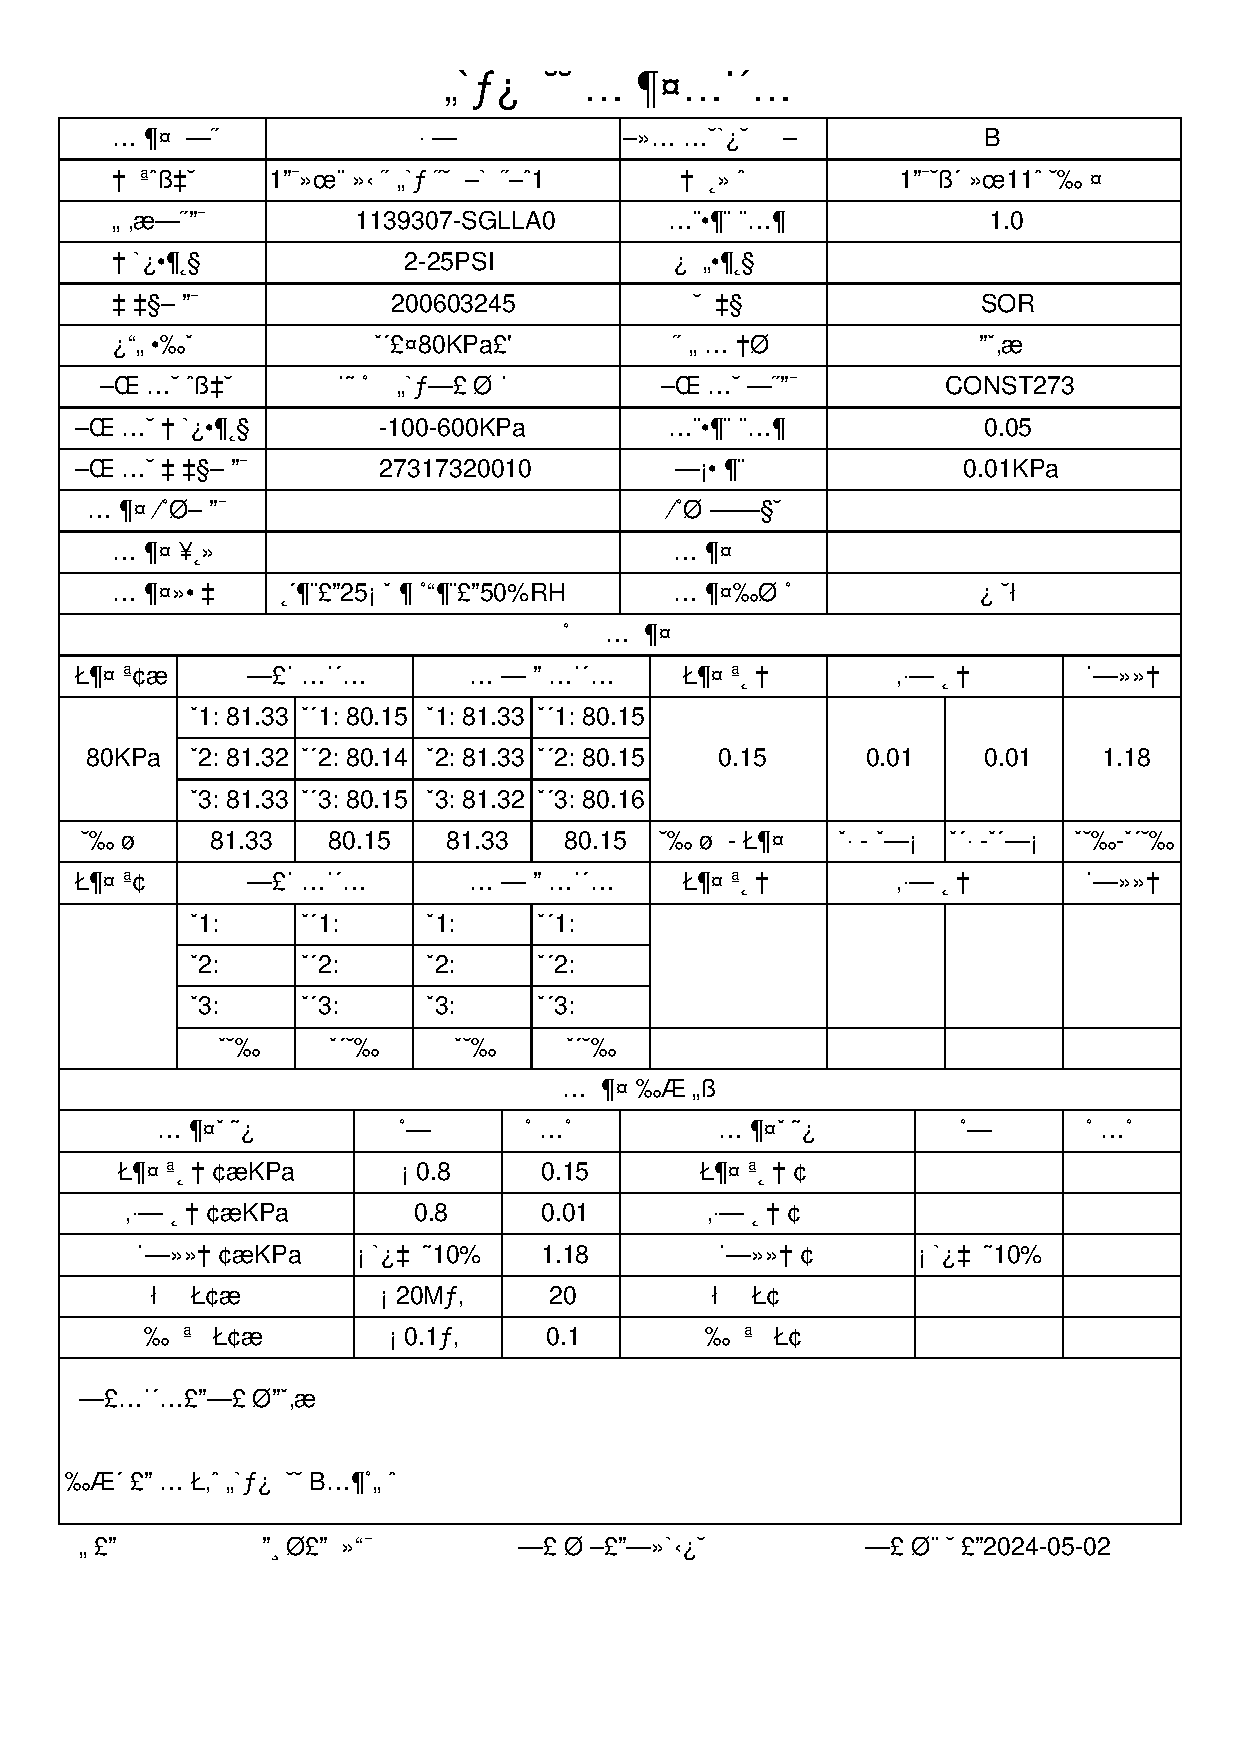
\includepdf[pages=-]{pdfpage.pdf}
% 单页 第一页
%\includepdf[pages={1}]{test1.pdf} 
% 单页 第5页
%\includepdf[pages={5}]{test1.pdf}
%  1,2,4页
%\includepdf[pages={1,2,4}]{test1.pdf}
%  1到3页
%\includepdf[pages={37-68}]{1.pdf}
%  多种方法结合, {}代表空页面
%\includepdf[pages={3,{},8-11,15}]{test1.pdf}
 
%合并pdf文档
% 完整合并
\end{document}
